\chapter{Data Transformation}
This section outlines the data preprocessing steps taken in our analysis. Various combinations of preprocessing steps were considered in this paper to explore the effect of the choice of preprocessing step has on the single model vs multistage question. This section provides an over view of what steps could be taken as well has how one would go about it. All results presented in the later \ref{chp:experiments} will include a description of the preprocessing choices made.

\section{Sequence construction}
The models were trained on input, target sequences constructed using a rolling window over the observed time series data. Sequences were created on a trace by trace basis, i.e. there is no 1 sequence that contains observations from 2 different traces. A pair of input, target sequences will herein be referred to as a sample observation.

For a given pair of input and target, the input sequence is the observed values of the predictor features over the past $p$ seconds. The target is the observed $DL\_bitrate$ of the next $k$ seconds. The variables $p$ and $k$ are referred to as the history and horizon window respectively. A single input sequence takes the shape of a [n x f] matrix where f is the no of features used to predict the target. A single target sequence takes the shape of a [k x 1] matrix as we are only interested in predicting $DL\_bitrate$. For example in the univariate case we used a history window of 10 seconds, a horizon window of 5 seconds. Previous values of $DL\_bitrate$ were used to predict the throughput horizon. E.g.
\begin{equation}
\begin{aligned}
 input&: [10 \times 1] \\
 target&: [5 \times 1]
\end{aligned}
\end{equation}

\section{Choice of History \& Horizon Windows}
A typical input for an Lstm model used in forecasting takes the shape of: $[ n, p, q ]$ where n is the number of examples, p is the length of the history window and q is the number of features. The output will then be in the form of $[n, k, s ]$ where k is the length of the horizon window and s is the number of target variables the model predicts, typically s=1. Fig \ref{fig:example_of_ts} illustrates the construction of a single example in the univariate case.

\begin{figure}[h]
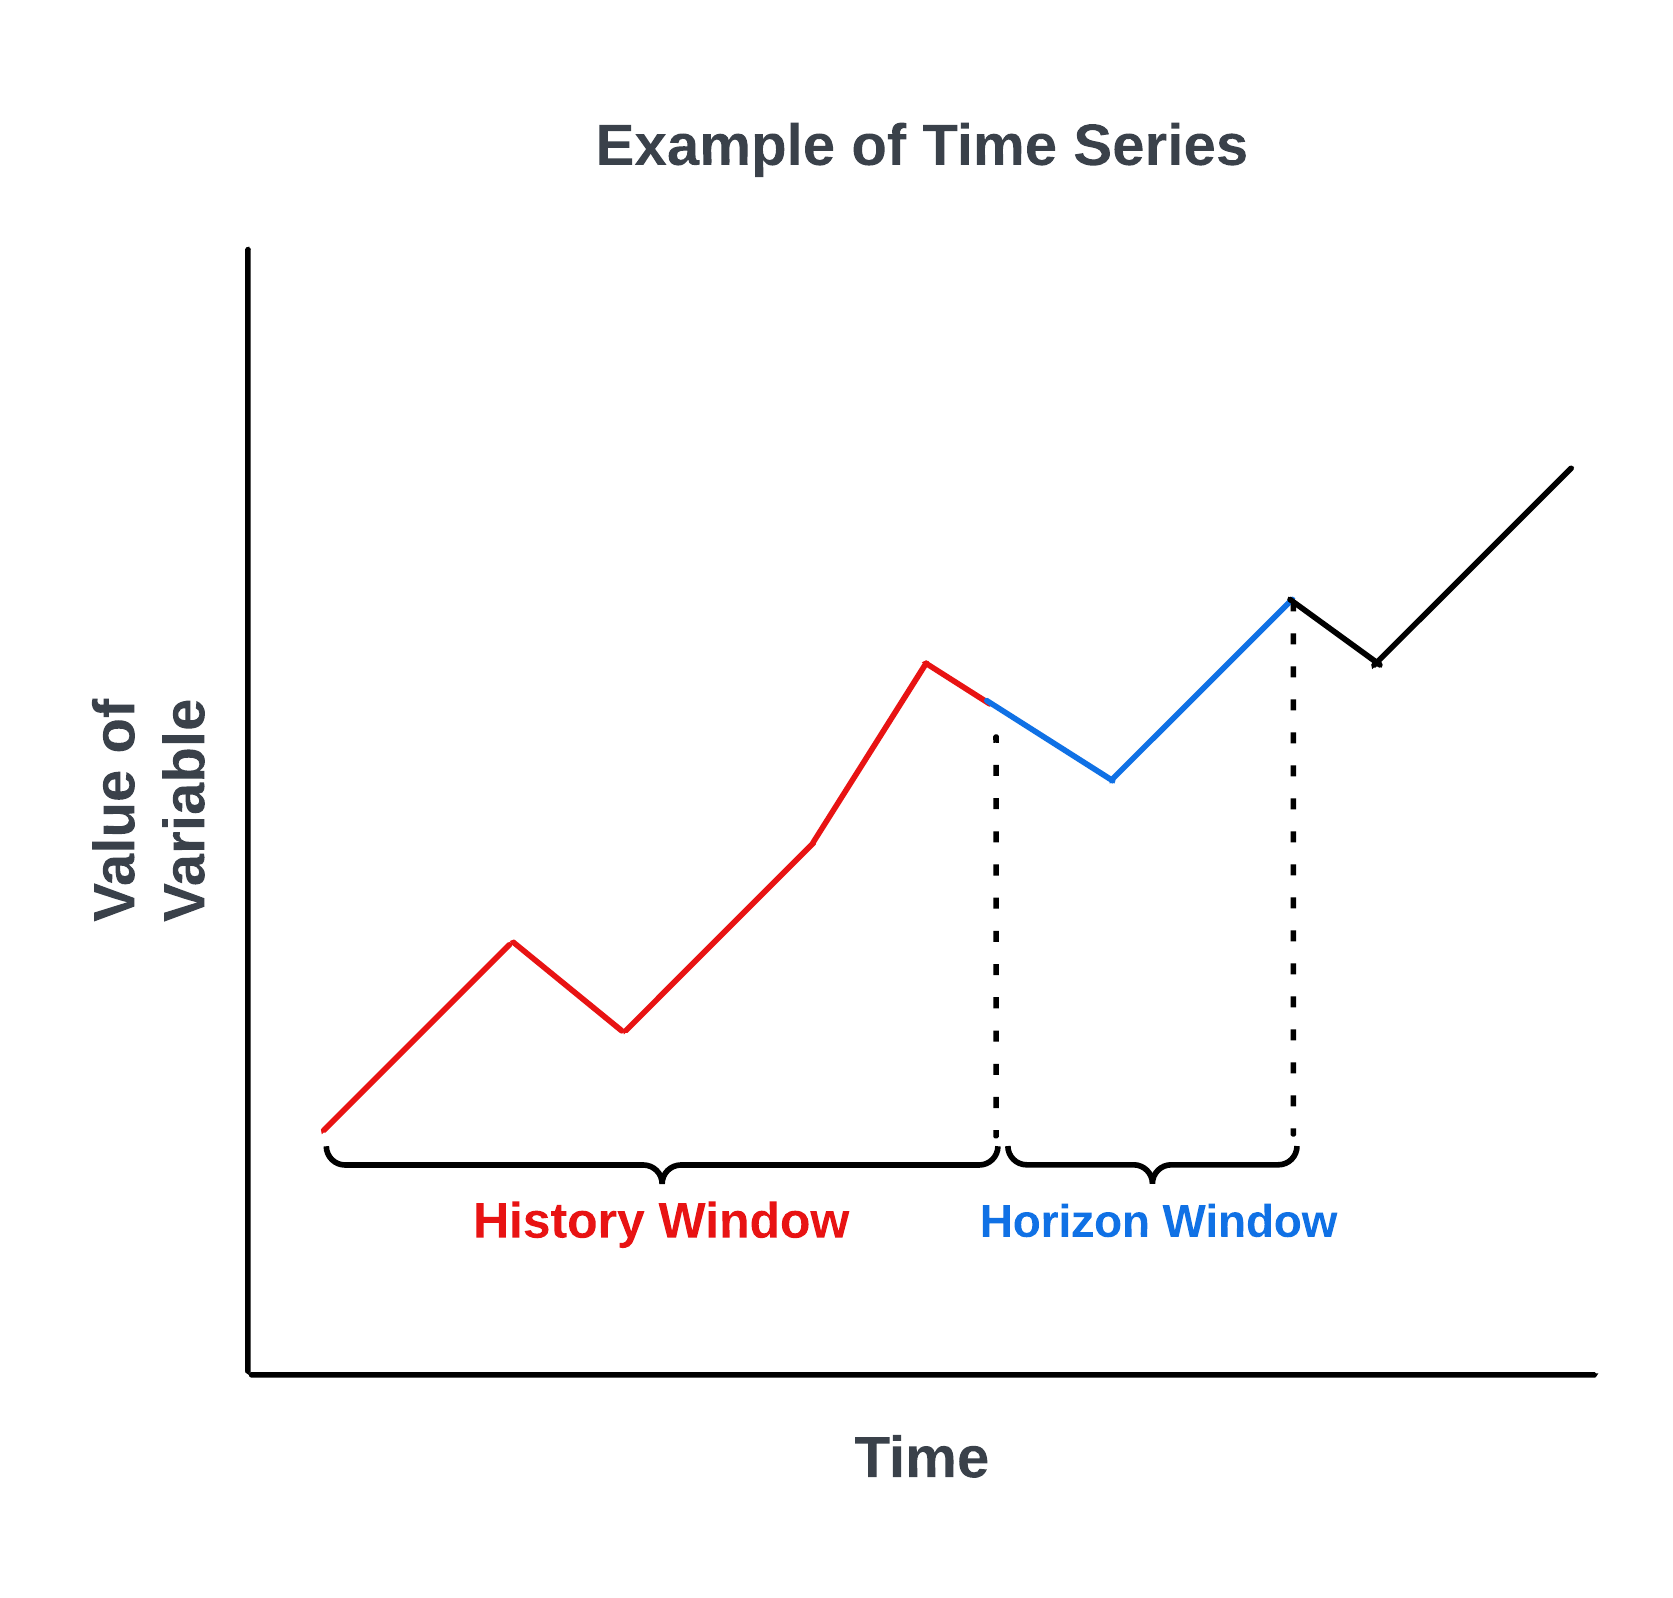
\includegraphics[scale=0.15]{History Horizon.png}
\centering
\caption{Graph showing how a history and horizon window can be constructed for a feature in time series data}
\label{fig:example_of_ts}
\end{figure}

There are many methods for identifying the optimal length of the horizon and history windows. Well studied methods such as the ACF (auto correlation function) or PACF (partial auto correlation function) \cite{10.2307/2958346} are useful for identifying temporal dependencies in the univariate case. The multivariate case is more complex as the target depends not only on previous values of itself, but previous values of other features. Still ACF provided a useful insight into the choices of history windows to consider. An ACF of <0.4 indicates that including values at the time lag does not contribute greatly to predicting the current value. An ACF >0.8 indicates that a particular lag is very relavant when predicting the current and future value of a metric.

Looking at figure \ref{fig:dl_acf} which shows the average ACF of the download throughput over the previous minute we observed that significant contributions to the prediction of current values falls off after 26 seconds. The red shaded region shows the standard deviation of the ACF observed over all traces. Intuitively this also suggests that for a horizon window of 5 seconds, 21 seconds would be an adequate maximum bound to consider for the history window. 

\begin{figure}[h]
\includegraphics[scale=0.5]{Images/Average_DL_bitrate_ACF.png}
\centering
\caption{This figure shows the average value of the auto correlation function for download throughput over all traces}
\label{fig:dl_acf}
\end{figure}

A selection of different combinations of horizon and history windows were considered to evaluate the impact each has on the throughput horizon predictions. The horizon window is more application dependent. The granularity of data available to us through G-NetTrack Pro is one second. In general more time sensitive applications such as web-conferencing would benefit a smaller horizon window. This incurs the cost of more computational power as the throughput prediction model must be run more frequently. Inversely, less time sensitive applications could use a longer horizon window. For throughput prediction, if the average horizon throughput is the main variable of interest then a longer horizon length may actually benefit predictions as the average will be calculated over a greater number of throughput predictions \cite{raca2019improving}.

\section{Selection of train/test Splits}
Typical train/test splits divide the dataset in a given ratio, usually 80:20 for train and test respectively. This is difficult to reproduce with this dataset as the dataset is not a single continuous time series but a collection of 135 distinct time series experiments. Train and test can be created by dividing the dataset based on the number of traces however, as seen in \ref{sec:distribution} the traces are of varying length making it difficult to split the dataset based on solo on the count. Instead, division of the traces was viewed an an optimisation problem. For each trace, the number of observations for each class of low, medium and high throughput was calculated. The number of observations of each class will vary based on the chosen horizon length and as such, different choices of horizon length will require a different train and test partition. The output of this process is as follows:
\begin{table}[!htb]
  \centering
  \caption{Example of Label Counting Output}
  \begin{tabular}{|c|c|c|c|}
    \hline
    Trace No. & Low Sequence Count & Medium Sequence Count & High Sequence Count \\
    \hline
    0 & 10 & 30 & 100 \\
    1 & 4 & 32 & 70\\
    2  & 0 & 60 & 130\\
    \hline
  \end{tabular}
\end{table}
The class counts per trace were then used to calculate a percentage of the total number of observations in each class over all traces contained within each trace. These percentages are then used partition the 135 traces in a given ratio (4:1 was used) in order to achieve the desired distribution of sequences in the train/test sets. Ideally the train set would include: \\
- 80\% of all low samples, 80\% of all medium samples and 80\% of all high samples \\
- Test would be the remainder i.e 20\% of low, medium and high \\

In practice it is difficult to find a split of traces that achieves the perfect ratio between low/medium/high for train and test. Instead a large number (10000) of potential splits are created and their class \% are measured. The split that is chosen is the train/test split with the lowest sum of differences between \% training low, medium, high, that is to say, train/test split chosen has the closest distribution to the desired distribution outlined above. The preprocessing code provides a summary of the distribution of the train/test split it finds. For example, most of the analysis in this paper focuses on a history window of 10 seconds and a horizon window of 5 seconds. The distribution of the train / test split for this selection is shown in table \ref 

\begin{table}[!htb]
  \centering
  \caption{Train/Test Class Distribution}
  \npdecimalsign{.}
  \nprounddigits{7}
  \begin{tabular}{|c|n{2}{7}|n{2}{7}|n{2}{7}|n{2}{7}|}
    \hline
    {Test Set} & {MSE} & {MAE} & {MAPE} & {Time to Predict (ms)} \\
    \hline
	All & 0.003487341 & 0.034651205 & 1.974610253 & 0.166163896\\
	Low & 0.000380131 & 0.013548465 & 0.678993196 & 0.170406616\\
	Medium & 0.00075947 & 0.017744765 & 0.902316831 & 0.156551365 \\
	High & 0.00591402 & 0.050246894 & 2.950865839 & 0.151185317 \\
    \hline
  \end{tabular}
  \npnoround
\end{table}

\section{Identifying Bounds for Mutlistage Model Classes}
\label{sec:bounds}
Two multistage approaches for modelling throughput prediction were considered in this paper. Each of the two architectures however share the same base models. Both multistage architectures proposed make use of a simple classifier that aims to predict a horizon throughput as one of 3 distinct situations, low throughput, medium throughput or high throughput. The choice to divide the problem based on the value of the download throughput comes from the fact that traces typically reported throughput above certain bounds (5Mbps, 1Mbps etc) far more often than below them. This imbalance leads to a single stage model frequently overestimating in low/medium throughput situations. Overestimating in these low or medium throughput scenarios leads to a noticeable decrease in the perceived quality of experience in applications such as video streaming \cite{raca2019improving} and is one of the main motivations of the multistage approach. 

The choice of the number of bounds (and subsequently models) and how to classify a given sequence of input data is arbitrary. For the purposes of this paper, dividing the data into one of three bounds sufficed. The sequences were divided by horizon download throughput into the three following ranges:

•Low: $ mean[y] < 1Mbps$ \\
•Medium: $1Mpbs \leq mean[y] \leq 5Mpbs$ \\
•High: $ mean[y] > 5Mbps$ \\

For forecasting, Lstm models are typically trained on x, y pairs where x is historic data of the predictor features over the past p seconds and y is the true value of the target variable of the next k seconds. The average download throughput of y was used to classify a given trace as an example of high, medium or low throughput.

The bounds 1Mbps and 5Mbps were chosen based on domain knowledge. Popular video streaming applications provide guidelines for the required download throughput for given video quality. As of the time of writing, 720p video requires 3Mbps on Netlfix whereas Youtube and Amazon Prime Video require at least 5Mbps of download throughput. While the adoption of AV1 hardware encoding may lower the required bitrate for HD video, use of the codec is still a while off mass market adoption and providers could choose to maintain the current bitrate while providing better quality source content.

\section{Feature Selection}
Feature selection is an important step in any machine learning problem. Good feature selection is known to improve loss, increase runtime performance and improve the understandability of predictions \cite{guyon2003introduction}.
Feature selection for multivariate time series is still an evolving field. The challenge is that the a selected feature set must capture the correlation between the target variable and predictors as well as between the target variable and lagged values of the predictors.

Feature selection is important for the analysis of multistage vs single stage throughput predictors explored this paper as it is an effective method in reducing the number of parameters of a given model. This is especially important when tight constraints are put on model size (in memory) and speed of inference, as is the case for models intended for mobile devices.

The number of feature included in the dataset is relatively small at 19 by current deep learning standards. This allows for methods such as exhaustive search to be viable, however hardware limitations prevented us from carrying out such an analysis due to time constraints. Geo-location data related to the serving cell tower was excluded from consideration. This data is currently not readily available on mobile devices and had to be gathered from a third party source \href{https://opencellid.org/}.

Firstly to explore the correlation between features. Fig \ref{fig:feature_correlation} shows the average correlation matrix over all traces. The features: RSRQ, RSSI, RSRP, NRxRSRP and NRxRSRQ are measured on a logarithmic scale and as such were transformed using the following formula before calculating the correlation matrix:
\begin{equation}
Y = exp(\left|X\right|)
\end{equation}
NetworkMode\_\{X\} is the one-hot-encoded transform of the NetworkMode feature, the same is true for State\_I and State\_DBefore performing this transform correlation between DL\_bitrate and these features was not observed. Understanding this matrix requires some careful thought. Firstly, this is a time series problem, DL\_bitrate will be used to predict itself. Knowing this, the observed strong correlation between DL\_bitrate and UL\_bitrate is misleading in regards to feature selection. This matrix suggests that including UL\_bitrate might actually be redundant. SNR and CQI are good candidates for inclusion in the optimal feature subset. RSRQ and NRxRSRP are also good candidates for inclusion. RSRQ has strong correlation with both CQI and SNR suggesting that one of either SNR or CQI could be also be dropped should constraints call for it. Geo-location data had no correlation with DL\_bitrate which is to be expected as the dataset was constructed from mobile devices in a relatively small geographic area. The NetworkMode variables were one-hot encoded and as such correlation is less applicable for these features. This matrix suggests that a good feature selection would include:

-DL\_bitrate \\
-SNR \\
-CQI \\
-NRxRSRP \\
-RSRQ \\

\newpage
\begin{figure}[h]
\includegraphics[scale=0.5]{Images/feature_correlation.png}
\centering
\caption{Correlation matrix showing the average correlation between features over all traces}
\label{fig:feature_correlation}
\end{figure}

Next permutation feature importance was considered. An Lstm was fit on all network related features, as well as location data for the mobile device. The Lstm used was the standard Lstm identfied in section \ref{sec:model_tuning} The metric we chose to compare the results of this test is the mean absolute percentage error (MAPE) given by the following formula: \\

\begin{equation}
MAPE = \frac{1}{n} \times \frac{\left|true-predicted\right|}{true} \times 100
\end{equation}
where $n$ is the number of observations in the test set.

The procedure for permutation feature importance is as follows:

- Given a target variable $Y$, with predictor variables $X=\{X_1,X_2,X_3,...X_n\}$ \\
- Create a train/test split of the dataset \\
- Fit a model on the training data using all features in $X$ \\
- Compute the loss of the model on the test set to use as a baseline \\
- Randomly shuffle the values of one feature $X_k$ in the test set and compute the loss with just this feature's values shuffled. Do this $\forall X_k \in X$. \\
- Compared the performance of the model on the test set with the performance of the model on each test set with a shuffled feature \\
- Rank the features based on the difference in performance \\
- Use this ranked list to identify possible features to eliminate \\

The results of this analysis can be seen in figure \ref{fig:feature_importance}. In this case the model relied heavily on the NetworkMode feature. RSRQ was once again important in improving prediction performance. 
\newpage
\begin{figure}[h]
\includegraphics[scale=0.5]{Images/feature_importance.png}
\centering
\caption{Bar Chart showing Difference in Model Performance with Permuted Feature Column.}
\label{fig:feature_importance}
\end{figure}